\section{Qualitative Variables Conditioned on Quantitative Densities}  

Often it is useful to find representative patterns (clusters) from sets of data. These clusters can in turn be considered categories of the groupings of quantitative data and the cluster membership yields the distribution of these categories. 

\begin{figure}
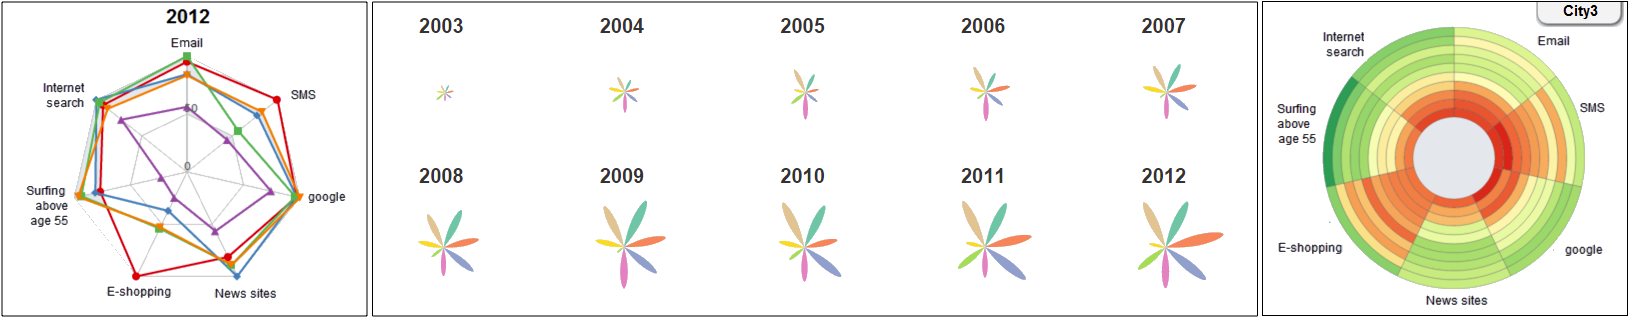
\includegraphics[width=1\textwidth]{radial}
\caption{Figure from \cite{albo_off_2016}. Radar chart, flower chart, and circle
  charts}
\label{fig:radial}
\end{figure}
Radial visualizations can be used to show representative
categories from multivariate vectors. For example, as seen in figure~\ref{fig:radial}
radar plot, the clusterings of the area types indicates general categories for
the data, and the number of areas in each cluster indicates the relative
frequency. Flower charts can also be grouped to find these relative
categories, as can the rings in a circle chart. Parallel coordinates charts are often explicitly grouped by category, but the relative frequency of the colors can be used to derive the relative frequencies of each graph. 

\begin{figure}
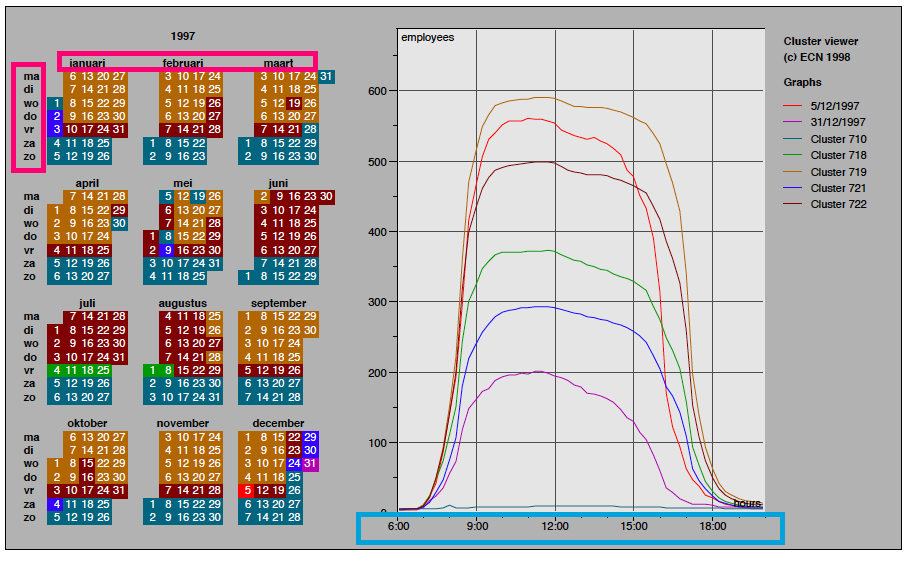
\includegraphics[width=1\textwidth]{calendar.png}
\caption{Figure from \cite{van_wijk_cluster_1999}. They visualized representative clusters of electricty usage and the relative frequency of each cluster using a calendar where day and cluster that day share the same color.}
\label{fig:calendar}
\end{figure}

Finding patterns and trends in large datasets, whether univariate or multivariate, is often a matter of trying to find representational fingerprints of common or outlying events in the dataset. This is frequently done through the use of a clustering algorithm. Figure~ref{fig:calendar} shows an analysis of electricity usage in the Netherlands\cite{van_wijk_cluster_1999}. Because the individual observations were recorded every 6 hours for a year, van Wilk and van Selow transformed the hourly observations into a matrix where each vector holds the observations for a given day. They used an agglomerative clustering algorithm \cite{kaufman_agglomerative_1990} to find representative days, and color matched these clusters to a calendar of days to visualize how these clusters were distributed over time. 

Techniques specifically aimed at clustering functional data can be found in the survey by Jacques, Julian and Preda \cite{Jacques_functional_2014}. %%todo: read and write up
